% knitr mixed latex en R tot pdf
\documentclass[10pt,a4paper,titlepage]{report}

\usepackage[latin1]{inputenc}
\usepackage[english]{babel}
\usepackage{amsmath}
\usepackage{amsfonts}
\usepackage{amssymb}
\usepackage{graphicx}
% bepaald marges van papier
\usepackage[left=2cm,right=2cm,top=2cm,bottom=2cm]{geometry}
% voor plaatsten van figure
\usepackage{float}
% voor tabellen
\usepackage{longtable}

% header and footer definition
\usepackage{fancyhdr}
\pagestyle{fancy}

\lhead{
\includegraphics[height=0.8cm]{dikw-logo.png}}
\chead{}
\rhead{\bfseries Data Analysis Report}
\lfoot{}
\cfoot{Data $>$ Information $>$ Knowledge $>$ Wisdom}
\rfoot{\thepage}
\renewcommand{\headrulewidth}{0.4pt}
\renewcommand{\footrulewidth}{0.4pt}

\author{Hugo Koopmans}
\title{Data Analysis Report}
\begin{document}
\SweaveOpts{concordance=TRUE}
\maketitle
\tableofcontents
\newpage
\section{Introduction}
This data analysis report is generated using R, R-studio and knitr to sweave R code and Latex into pdf format. We have the option to include all R code that is used to generate the plots and calculations. Default this feauture is dissabled.\\
The data analysis step is the first step an a datamining analysis.
\section{Dataset Basic Artifacts}

\subsection{Basic dataset information}
Basic information on dataset:\\






\\
Read data from file : d5.tab.\\
The dataset has 37 variables and 59992 rows.

The case identifyer is registrnr this is unique for all cases.

\subsection{Excluded variables}
From the varables provided the folowing list will be excluded in this anlysis: caseID, registrnr, X2011tmoktstornaant, X2010stornoaantal

\subsection{Variabele types}


The following variabele are present in the dataset:\\
jaarbedr, minbegjr, proj, nudona, r20102009mndbedrag, r20112010mndbedrag, X2009avgbedragmnd, X2010avgbedragmnd, X2011avgbedragmnd, bronaktie, bronlaatstebetwijze, Jaarbinnen, sexe, leeftijd2011, Bronbinnen, mailingen, magpost, magdigi, diginws, TM, mail07, catHHINKOMEN, catHHSOCIALE, catHHOPLEIDI, catHHLEVENSF, catHHGEOTYPE, catHHTYPEWO, catHHEIGENDO, catHHWOZWAA, catBELEGGERS, catLENERS, catSPAARDERS, catSWITCHGEVO, catMERKENTROU 
\\
Sometimes categoric variables are present as coded numbers. These should be treated as factors.
In this dataset the following variables will be used as factors(categoric): catHHINKOMEN, catHHSOCIALE, catHHOPLEIDI, catHHLEVENSF, catHHGEOTYPE, catHHTYPEWO, catHHEIGENDO, catHHWOZWAA, catBELEGGERS, catLENERS, catSPAARDERS, catSWITCHGEVO, catMERKENTROU
\\
We have 13 numeric variables and 21 categorical variables (or factors in R).
\newpage
\section{Numeric variables}
Here we analyse all numeric variables. We start with an overview on basic statistics per variable. We check for missing values. We do a histogram plot to show the distribution for this variable. And we test for outliers.

\subsection{Overview}
In the table below we report the number of observations (n), the smallest observation (min),  the first quantile (q1), the media ,  the mean, last quantile, the largest observation (max), and the nber of missing values (na).\\

\begin{knitrout}
\definecolor{shadecolor}{rgb}{0.969, 0.969, 0.969}\color{fgcolor}\begin{kframe}


{\ttfamily\noindent\itshape\color{messagecolor}{\#\# Loading required package: xtable}}

{\ttfamily\noindent\itshape\color{messagecolor}{\#\# Loading required package: survival}}

{\ttfamily\noindent\itshape\color{messagecolor}{\#\# Loading required package: splines}}\begin{verbatim}
## % latex table generated in R 2.14.1 by xtable 1.7-1 package
## % Mon May 27 21:51:41 2013
## {\footnotesize
## \begin{longtable}{lrrrrrrrr}
##  \textbf{Variable} & $\mathbf{n}$ & \textbf{Min} & $\mathbf{q_1}$ & $\mathbf{\widetilde{x}}$ & $\mathbf{\bar{x}}$ & $\mathbf{q_3}$ & \textbf{Max} & \textbf{\#NA} \\ 
##   \hline
## jaarbedr & 59992 &    0.0 &   60 &   60 &   79.2 &   72.0 & 4898.8 &     0 \\ 
##   minbegjr & 59992 & 1900.0 & 1999 & 2008 & 2003.2 & 2009.0 & 2011.0 &     0 \\ 
##   proj & 59992 &    0.0 &    0 &    0 &    0.3 &    1.0 &   14.0 &     0 \\ 
##   nudona & 59992 &    0.0 &    1 &    1 &    0.9 &    1.0 &    1.0 &     0 \\ 
##   r20102009mndbedrag & 48938 &    0.0 &    1 &    1 &    1.0 &    1.0 &   11.2 & 11054 \\ 
##   r20112010mndbedrag & 55821 &    0.0 &    1 &    1 &    1.0 &    1.0 &   12.9 &  4171 \\ 
##   X2009avgbedragmnd & 49090 &    0.1 &    5 &    5 &    6.4 &    6.0 &  459.0 & 10902 \\ 
##   X2010avgbedragmnd & 55868 &    0.0 &    5 &    5 &    6.4 &    6.0 &  544.2 &  4124 \\ 
##   X2011avgbedragmnd & 59873 &    0.1 &    5 &    5 &    6.6 &    6.7 &  481.2 &   119 \\ 
##   Jaarbinnen & 59443 & 1988.0 & 1990 & 2006 & 2000.8 & 2009.0 & 2011.0 &   549 \\ 
##   leeftijd2011 & 41620 &    4.0 &   41 &   52 &   53.2 &   65.0 &  111.0 & 18372 \\ 
##   mailingen & 59443 &    0.0 &   99 &   99 &   86.2 &   99.0 &   99.0 &   549 \\ 
##   magpost & 59443 &    0.0 &    9 &    9 &    8.0 &    9.0 &    9.0 &   549 \\ 
##   \hline
## \caption{} 
## \label{}
## \end{longtable}
## }
\end{verbatim}
\end{kframe}
\end{knitrout}


 



% child template for numeric variables

\subsection{Variabele jaarbedr}
%\textbf{Variabele num_var_names[i]}

Missing :  0 \\
Minimum value : 0\\
Percentile 1 : 10\\
Percentile 99 : 300\\
Maximum value : 4898.8

\color{red}
Warning : Suspect extreme values in left tailWarning : Suspect extreme values in right tail

\color{black}

\begin{figure}[H]
   \centering
\begin{knitrout}
\definecolor{shadecolor}{rgb}{0.969, 0.969, 0.969}\color{fgcolor}
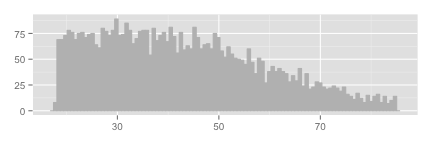
\includegraphics[width=\maxwidth]{figure/unnamed-chunk-2} 

\end{knitrout}

    \caption{Histogram jaarbedr}
    \label{fig:figPlot1}
\end{figure}

% child template for numeric variables

\subsection{Variabele minbegjr}
%\textbf{Variabele num_var_names[i]}

Missing :  0 \\
Minimum value : 1900\\
Percentile 1 : 1900\\
Percentile 99 : 2011\\
Maximum value : 2011

\color{red}


\color{black}

\begin{figure}[H]
   \centering
\begin{knitrout}
\definecolor{shadecolor}{rgb}{0.969, 0.969, 0.969}\color{fgcolor}\begin{kframe}


{\ttfamily\noindent\color{warningcolor}{\#\# Warning: position\_stack requires constant width: output may be incorrect}}\end{kframe}
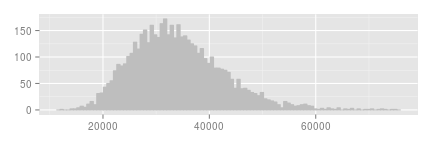
\includegraphics[width=\maxwidth]{figure/unnamed-chunk-4} 

\end{knitrout}

    \caption{Histogram minbegjr}
    \label{fig:figPlot2}
\end{figure}

% child template for numeric variables

\subsection{Variabele proj}
%\textbf{Variabele num_var_names[i]}

Missing :  0 \\
Minimum value : 0\\
Percentile 1 : 0\\
Percentile 99 : 1\\
Maximum value : 14

\color{red}
Warning : Suspect extreme values in right tail

\color{black}

\begin{figure}[H]
   \centering
\begin{knitrout}
\definecolor{shadecolor}{rgb}{0.969, 0.969, 0.969}\color{fgcolor}
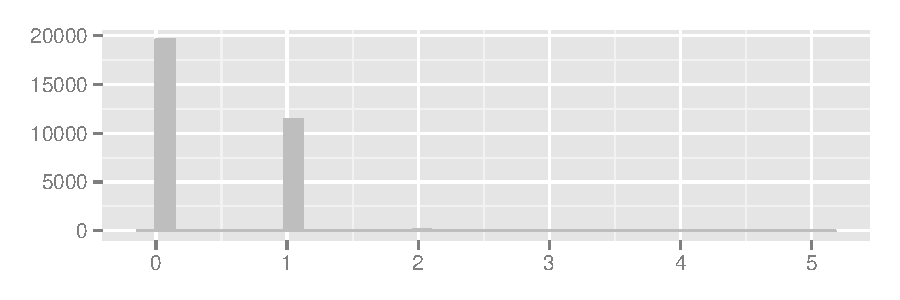
\includegraphics[width=\maxwidth]{figure/unnamed-chunk-6} 

\end{knitrout}

    \caption{Histogram proj}
    \label{fig:figPlot3}
\end{figure}

% child template for numeric variables

\subsection{Variabele nudona}
%\textbf{Variabele num_var_names[i]}

Missing :  0 \\
Minimum value : 0\\
Percentile 1 : 0\\
Percentile 99 : 1\\
Maximum value : 1

\color{red}


\color{black}

\begin{figure}[H]
   \centering
\begin{knitrout}
\definecolor{shadecolor}{rgb}{0.969, 0.969, 0.969}\color{fgcolor}\begin{kframe}


{\ttfamily\noindent\color{warningcolor}{\#\# Warning: position\_stack requires constant width: output may be incorrect}}\end{kframe}
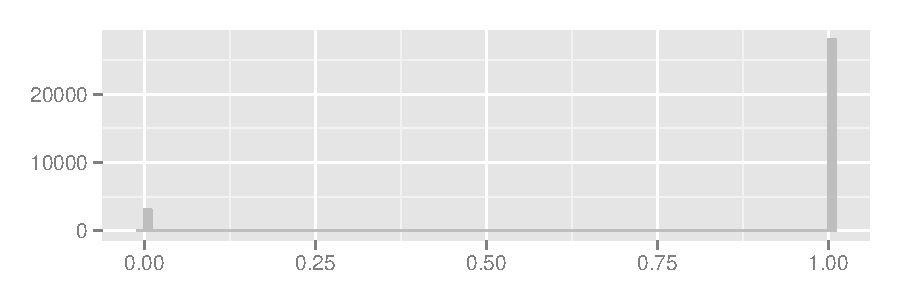
\includegraphics[width=\maxwidth]{figure/unnamed-chunk-8} 

\end{knitrout}

    \caption{Histogram nudona}
    \label{fig:figPlot4}
\end{figure}

% child template for numeric variables

\subsection{Variabele r20102009mndbedrag}
%\textbf{Variabele num_var_names[i]}

Missing :  11054 \\
Minimum value : 0.0463\\
Percentile 1 : 0.7\\
Percentile 99 : 1.4\\
Maximum value : 11.25

\color{red}
Warning : Suspect extreme values in left tailWarning : Suspect extreme values in right tail

\color{black}

\begin{figure}[H]
   \centering
\begin{knitrout}
\definecolor{shadecolor}{rgb}{0.969, 0.969, 0.969}\color{fgcolor}\begin{kframe}


{\ttfamily\noindent\color{warningcolor}{\#\# Warning: position\_stack requires constant width: output may be incorrect}}\end{kframe}
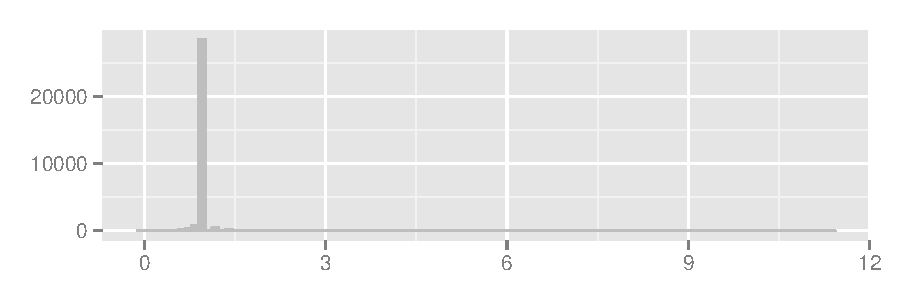
\includegraphics[width=\maxwidth]{figure/unnamed-chunk-10} 

\end{knitrout}

    \caption{Histogram r20102009mndbedrag}
    \label{fig:figPlot5}
\end{figure}

% child template for numeric variables

\subsection{Variabele r20112010mndbedrag}
%\textbf{Variabele num_var_names[i]}

Missing :  4171 \\
Minimum value : 0.0198\\
Percentile 1 : 0.5556\\
Percentile 99 : 2.1778\\
Maximum value : 12.9231

\color{red}
Warning : Suspect extreme values in left tailWarning : Suspect extreme values in right tail

\color{black}

\begin{figure}[H]
   \centering
\begin{knitrout}
\definecolor{shadecolor}{rgb}{0.969, 0.969, 0.969}\color{fgcolor}
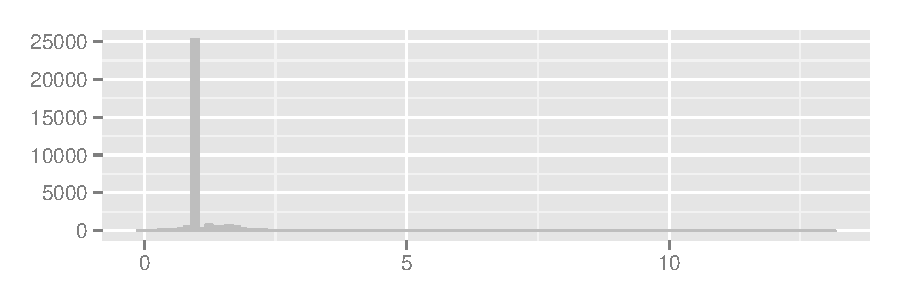
\includegraphics[width=\maxwidth]{figure/unnamed-chunk-12} 

\end{knitrout}

    \caption{Histogram r20112010mndbedrag}
    \label{fig:figPlot6}
\end{figure}

% child template for numeric variables

\subsection{Variabele X2009avgbedragmnd}
%\textbf{Variabele num_var_names[i]}

Missing :  10902 \\
Minimum value : 0.0625\\
Percentile 1 : 0.8333\\
Percentile 99 : 25\\
Maximum value : 459

\color{red}
Warning : Suspect extreme values in left tailWarning : Suspect extreme values in right tail

\color{black}

\begin{figure}[H]
   \centering
\begin{knitrout}
\definecolor{shadecolor}{rgb}{0.969, 0.969, 0.969}\color{fgcolor}
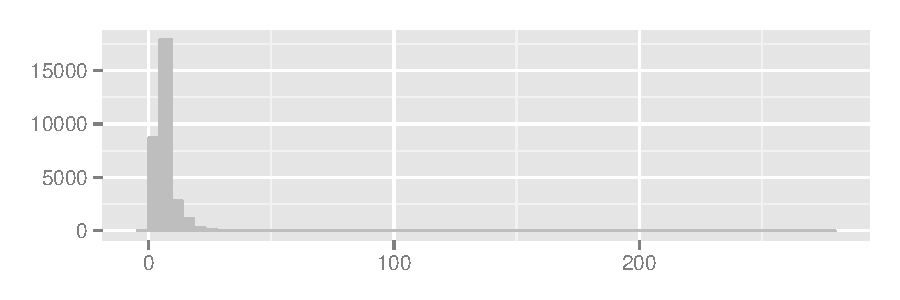
\includegraphics[width=\maxwidth]{figure/unnamed-chunk-14} 

\end{knitrout}

    \caption{Histogram X2009avgbedragmnd}
    \label{fig:figPlot7}
\end{figure}

% child template for numeric variables

\subsection{Variabele X2010avgbedragmnd}
%\textbf{Variabele num_var_names[i]}

Missing :  4124 \\
Minimum value : 0.025\\
Percentile 1 : 0.8333\\
Percentile 99 : 25\\
Maximum value : 544.2427

\color{red}
Warning : Suspect extreme values in left tailWarning : Suspect extreme values in right tail

\color{black}

\begin{figure}[H]
   \centering
\begin{knitrout}
\definecolor{shadecolor}{rgb}{0.969, 0.969, 0.969}\color{fgcolor}
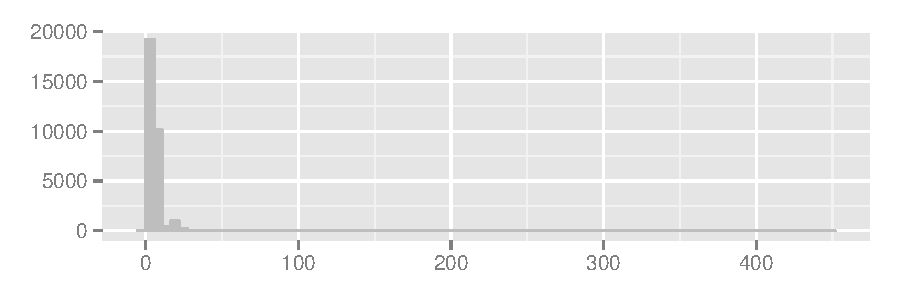
\includegraphics[width=\maxwidth]{figure/unnamed-chunk-16} 

\end{knitrout}

    \caption{Histogram X2010avgbedragmnd}
    \label{fig:figPlot8}
\end{figure}

% child template for numeric variables

\subsection{Variabele X2011avgbedragmnd}
%\textbf{Variabele num_var_names[i]}

Missing :  119 \\
Minimum value : 0.0595\\
Percentile 1 : 0.8333\\
Percentile 99 : 25\\
Maximum value : 481.25

\color{red}
Warning : Suspect extreme values in left tailWarning : Suspect extreme values in right tail

\color{black}

\begin{figure}[H]
   \centering
\begin{knitrout}
\definecolor{shadecolor}{rgb}{0.969, 0.969, 0.969}\color{fgcolor}
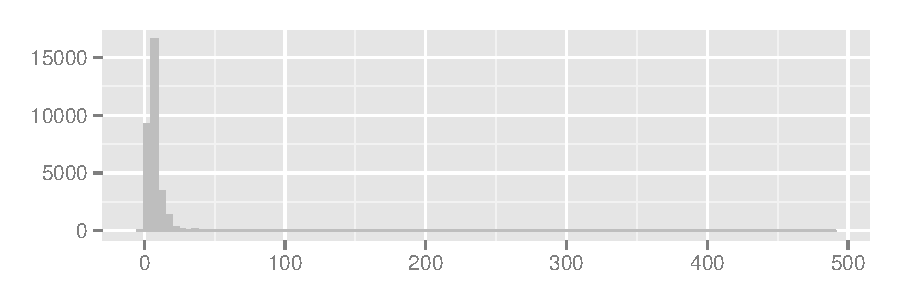
\includegraphics[width=\maxwidth]{figure/unnamed-chunk-18} 

\end{knitrout}

    \caption{Histogram X2011avgbedragmnd}
    \label{fig:figPlot9}
\end{figure}

% child template for numeric variables

\subsection{Variabele Jaarbinnen}
%\textbf{Variabele num_var_names[i]}

Missing :  549 \\
Minimum value : 1988\\
Percentile 1 : 1988\\
Percentile 99 : 2011\\
Maximum value : 2011

\color{red}


\color{black}

\begin{figure}[H]
   \centering
\begin{knitrout}
\definecolor{shadecolor}{rgb}{0.969, 0.969, 0.969}\color{fgcolor}\begin{kframe}


{\ttfamily\noindent\color{warningcolor}{\#\# Warning: position\_stack requires constant width: output may be incorrect}}\end{kframe}
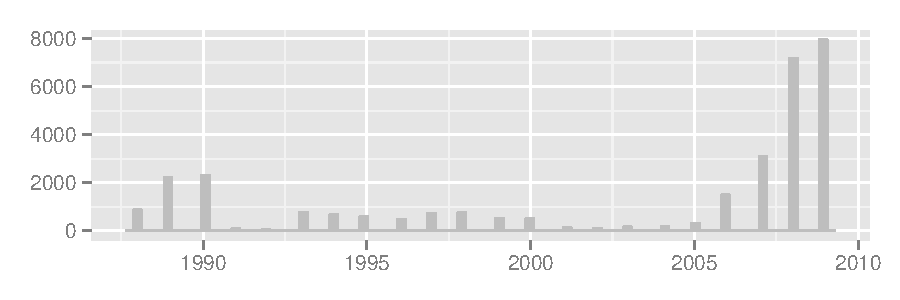
\includegraphics[width=\maxwidth]{figure/unnamed-chunk-20} 

\end{knitrout}

    \caption{Histogram Jaarbinnen}
    \label{fig:figPlot10}
\end{figure}

% child template for numeric variables

\subsection{Variabele leeftijd2011}
%\textbf{Variabele num_var_names[i]}

Missing :  18372 \\
Minimum value : 4\\
Percentile 1 : 21\\
Percentile 99 : 90\\
Maximum value : 111

\color{red}
Warning : Suspect extreme values in left tail

\color{black}

\begin{figure}[H]
   \centering
\begin{knitrout}
\definecolor{shadecolor}{rgb}{0.969, 0.969, 0.969}\color{fgcolor}
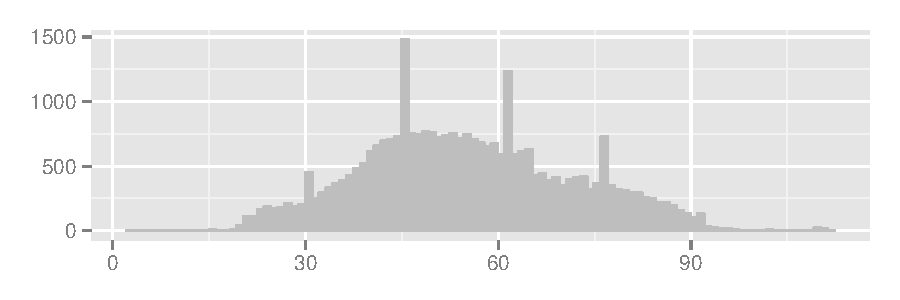
\includegraphics[width=\maxwidth]{figure/unnamed-chunk-22} 

\end{knitrout}

    \caption{Histogram leeftijd2011}
    \label{fig:figPlot11}
\end{figure}

% child template for numeric variables

\subsection{Variabele mailingen}
%\textbf{Variabele num_var_names[i]}

Missing :  549 \\
Minimum value : 0\\
Percentile 1 : 0\\
Percentile 99 : 99\\
Maximum value : 99

\color{red}


\color{black}

\begin{figure}[H]
   \centering
\begin{knitrout}
\definecolor{shadecolor}{rgb}{0.969, 0.969, 0.969}\color{fgcolor}
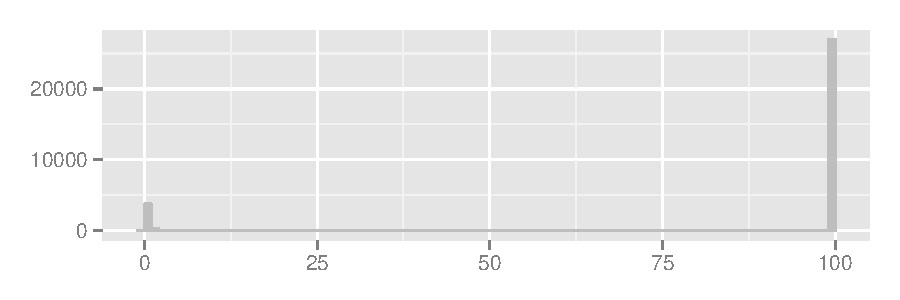
\includegraphics[width=\maxwidth]{figure/unnamed-chunk-24} 

\end{knitrout}

    \caption{Histogram mailingen}
    \label{fig:figPlot12}
\end{figure}

% child template for numeric variables

\subsection{Variabele magpost}
%\textbf{Variabele num_var_names[i]}

Missing :  549 \\
Minimum value : 0\\
Percentile 1 : 0\\
Percentile 99 : 9\\
Maximum value : 9

\color{red}


\color{black}

\begin{figure}[H]
   \centering
\begin{knitrout}
\definecolor{shadecolor}{rgb}{0.969, 0.969, 0.969}\color{fgcolor}\begin{kframe}


{\ttfamily\noindent\color{warningcolor}{\#\# Warning: position\_stack requires constant width: output may be incorrect}}\end{kframe}
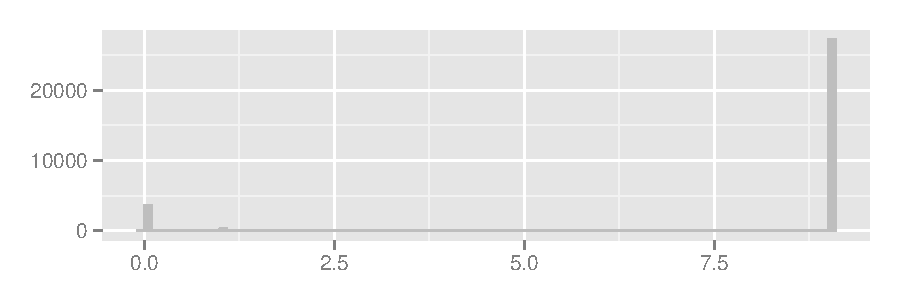
\includegraphics[width=\maxwidth]{figure/unnamed-chunk-26} 

\end{knitrout}

    \caption{Histogram magpost}
    \label{fig:figPlot13}
\end{figure}


% analyse categorical variabels
\newpage
\section{Categorical variables}
Here we analyse all categorical variables. We first check the number of different levels in each category(or factor). Then we do a bar plot to show the distribution for each variable.
\\
Overview\\
In the following table we will see each variable printed with it's unique levels. Beside each level a count is made and a precentage calculated. In the last colum we find a culumative count summing the total up to 100\%. 


We see that the number of levels can be quite big, for reporting we will omit all variables with more then  25 levels. These will not be reported in the subsections below.
\begin{knitrout}
\definecolor{shadecolor}{rgb}{0.969, 0.969, 0.969}\color{fgcolor}\begin{kframe}
\begin{verbatim}
## % latex table generated in R 2.14.1 by xtable 1.7-1 package
## % Mon May 27 21:51:48 2013
## \begin{table}[ht]
## \centering
## \begin{tabular}{rrr}
##   \hline
##  & levels & \# missings \\ 
##   \hline
## bronaktie & 403 & 0 \\ 
##   bronlaatstebetwijze & 11 & 0 \\ 
##   sexe & 5 & 0 \\ 
##   Bronbinnen & 11 & 0 \\ 
##   magdigi & 3 & 0 \\ 
##   diginws & 3 & 0 \\ 
##   TM & 3 & 0 \\ 
##   mail07 & 3 & 0 \\ 
##   catHHINKOMEN & 7 & 0 \\ 
##   catHHSOCIALE & 6 & 0 \\ 
##   catHHOPLEIDI & 4 & 0 \\ 
##   catHHLEVENSF & 10 & 0 \\ 
##   catHHGEOTYPE & 21 & 0 \\ 
##   catHHTYPEWO & 11 & 0 \\ 
##   catHHEIGENDO & 3 & 0 \\ 
##   catHHWOZWAA & 13 & 0 \\ 
##   catBELEGGERS & 10 & 0 \\ 
##   catLENERS & 10 & 0 \\ 
##   catSPAARDERS & 10 & 0 \\ 
##   catSWITCHGEVO & 10 & 0 \\ 
##   catMERKENTROU & 10 & 0 \\ 
##    \hline
## \end{tabular}
## \end{table}
\end{verbatim}
\end{kframe}
\end{knitrout}


Variables with to many levels to report are : 





